\chapter{Molecular Dynamics}

Molecular dynamics simulations is an umbrella term for a class of
computational methods used to model and analyze the physical behavior of
systems of atoms and molecules. MD allows one to monitor the full time
evolution of a system, allowing for deep examination of the dynamics of
atomic-level phenomena that cannot be observed directly.
Computer simulations applied to condensed matter systems began their
development as early as the 1950s, when two of the pillars of molecular
simulation were introduced, namely the Monte Carlo (MC) sampling technique and
the molecular dynamics method. In 1964, the first realistic MD simulation was
developed by Rahman, who came up with a realistic model of liquid argon
\cite{PhysRev.136.A405}. Rahman used the Lennard–Jones pair-wise additive
potential and showed, that MD simulations with smooth potentials were
possible.

Around the same time, Verlet proposed a stable numerical integration
algorithm that is still very popular in modern MD software
\cite{PhysRev.159.98}. We will discuss the Verlet integration algorithm in
further chapters of this thesis. Verlet also invented a time-saving algorithm,
the Verlet neighbour list.

A great leap forward in the MD methology happened in 1971, when Rahman and
Stillinger published an MD study on modeling a realistic system of liquid
water \cite{10.1063/1.1676585}. The significant results of their work prompted
a multinational group of scientists centred around Berendsen at CECAM to try
using MD simulations for examining biomolecules. The first MD simulation of a
simple protein was due to Karplus and collaborators, and appeared shortly
after, in 1977 \cite{McCammon1977-dx}. In 2013, the Nobel Prize for Chemistry
was awarded to Warshel, Levitt, and Karplus for their work on computer
simulations in biochemistry, which was built upon the efforts of many
researchers who had previously worked on simulating biomolecules.

Another inportant development took place in 1980. In this year, Anderson
published a paper that described how to extend MD to enable it to sample the
isoenthalpic (constant pressure) ensemble \cite{10.1063/1.439486}. The
standard molecular dynamics algorithm was designed to simulate the behavior of a system of particles at
constant energy, or in the microcanonical ensemble, because the Newton's
equations of motion conserve energy. It was not straightforward to modify the
MD algorithm to sample systems under different, more experimentally relevant
conditions. Andersen's extensions for sampling the isoenthalpic ensemble
inspired the question of whether it was possible to use MD to sample the
canonical ensemble as well. Nosé, building on Andersen's work, introduced a
new variable that linked the kinetic energy of the atoms to the external
temperature, resulting in dynamics that sample the desired ensemble. This
approach is known as the Nosé–Hoover thermostat, which is often used in a
modified form called the Hoover thermostat \cite{PhysRevA.31.1695}.

In 1985, Car and Parrinello published a groundbreaking paper in Physical
Review Letters that described a method for combining MD with density
functional theory (DFT) calculations of electronic structure \cite{pmid10032153}. This approach eliminated the need for a potential model,
as energy, forces, and stress could be calculated directly from the electronic
structure. The Car–Parrinello method allowed for the simulation of processes that involve bond formation or
breaking and was the first to demonstrate that it is possible to combine
finite temperature simulations with ground-state electronic structure
calculations. This method also served as a bridge between the simulation
community, which typically has a background in statistical mechanics, and the
solid-state physics and quantum chemistry communities, which focus on
electronic structure calculations at zero temperature.

During the 1980s and 1990s, the use of molecular simulations in condensed
matter research became more widespread, due in part to previous successes in
this field and also to the increasing availability and power of computers.

Modern MD methodology is frequently used to refine the three-dimensional
structures of proteins and other large molecules, to study atomic-level
phenomena that cannot be directly observed, such as thin-film growth and ion
implantation, and to investigate the physical properties of nanotechnological
devices that cannot yet be manufactured. In 2015, for example, MD simulation
has been reported for pharmacophore development and drug design \cite{pmid25751016}.

\section{Classical Methods}

The classical MD implementation uses the so-called "ball and sticks" model,
where atoms and molecules are treated as soft balls and their bonds are
represented by elastic sticks. The laws of classical mechanics define the
dynamics of the entire system.

Each particle in an MD simulation has its own position vector
$\mathbf{r}_i(t) = (x_i(t), y_i(t), z_i(t))$. A particle usually corresponds
to an atom, although it may represent any simulable entity of interest that
can be conveniently described by an interaction law. By Newton's second law
the motion of each particle must obey the following relation
\begin{equation}
  \mathbf{F}_i = m_i \diff[2]{\mathbf{r}_i}{t},
\end{equation}
where $m_i$ is the mass of $i$-th particle and $\mathbf{F}_i$ is the
force acting upon $i$-th particle. Interaction laws are usually specified by
a potential function $U(\mathbf{r}_1, \dots, \mathbf{r}_N)$, which represents
the potential energy of $N$ interacting particles as a function of their
positions. Given the potential, the force acting upon $i$-th atom is
determined by the gradient with respect to particle displacements
\begin{equation}
  \mathbf{F}_i = - \nabla_{\mathbf{r}_i} U(\mathbf{r}_1, \dots, \mathbf{r}_N)
  = - \left(
    \frac{\partial U}{\partial x_i},
    \frac{\partial U}{\partial y_i},
    \frac{\partial U}{\partial z_i}
  \right).
\end{equation}

Let's briefly talk about the meaning and form of the potential $U$
in MD simulations. Any quantum-chemistry textbook would insist, that in order
to appropriately examine a behavior of molecule, we can not just look at its
individual atoms. The quantum-mechanical lense reveals, that when atoms bond
into molecules, their electron orbitals interact in complex ways, giving rise
to non-trivial molecule orbitals. These electronic clouds that span multiple
atoms then determine molecule's interactions with other particles. This paints
molecules as a very complicated quantum systems, where electrons and nuclei
are interacting together in an intricate manner. It turns out, however, that
to a very good approximation, known as the Born–Oppenheimer adiabatic
approximation and based on the difference in mass between nuclei and
electrons, the electronic and nuclear problems can be separated. According to
this approximation, we can presume that the electron clouds equilibrate
quickly for each instanteneous configuration of the heavy nuclei. The nuclei
then move in the field created by the average electron densities.
This allows us to consider the concept of a potential energy surface, which
controls the movement of the nuclei without taking explicit account of the
electrons. Given the potential energy surface, we may use classical mechanics
to follow the dynamics of the nuclei. Rather than solving the
quantum-mechanical problem, we can solve a classic-mechanical problem, in
which the effect of the electrons on nuclei is expressed by en empirical
potential. It can be very challenging to identify a potential function that
accurately represents an energy surfaces of a system, but doing so greatly
simplifies the computational process. Atomic force field models and the
classical MD are based on empirical potentials with a specific functional
form, representing the physics and chemistry of the systems of
interest. The following equation is an example of such a force field, used in
biosystem simulations \cite{doi0003048}
\begin{equation}
\begin{alignedat}{2}
  U(\mathbf{r}_1, \dots, \mathbf{r}_N) = &
  \sum_\text{bonds} \frac{a_i}{2} (l_i - l_{i0})^2
  + \sum_\text{angles} \frac{b_i}{2} (\theta_i - \theta_{i0})^2 \\
  &+ \sum_\text{torsions} \frac{c_i}{2} \left[
    1 + \cos(n \omega_i - \gamma_i)
  \right] \\
  &+ \sum_\text{atom pairs} 4 \varepsilon_{ij} \left[
    \left(\frac{\sigma_{ij}}{r_{ij}}\right)^{12}
    - \left(\frac{\sigma_{ij}}{r_{ij}}\right)^{6}
  \right] \\
  &+ \sum_\text{atom pairs} k \frac{q_i q_j}{r_{ij}}.
\end{alignedat}
\end{equation}
The covalent character of the system is defined by the first three terms of
the system, where the summation indices run over all the bonds, angles and
torsions. In contrast, the last two terms are only defined by atom pairs,
with $q_i q_j$ being the product of their charges and $r_{ij} = |r_i - r_j|$
is the distance between the two atoms in the pair. The first two terms give
energies of deformations of the bond lengths $l_i$ and bond angles $\theta_i$
from their respective equilibrium values $l_{i0}$ and $\theta_{i0}$ with force
constants $a_i$ and $b_i$. These two terms model the correct chemical
structure, but prevent more complicated chemical phenomena like bond breaking.
Rotations around the chemical bond are described by the third therm, which is
priodic with periodicity determined by $n$ and heights of rotational barriers
defined by $c_i$. The forth term represents the van der Waals repulsive and
attractive interatomic forces in the form of the Lennard–Jones 12-6 potential.
The last term is the Coulomb electrostatic potential. Some effects due to
specific environments can be accounted for by properly adjusting partial
charges $q_i$ and effective value of the constant $k$ as well as the van der
Waals parameters $\varepsilon_{ij}$ and $\sigma_{ij}$.

We now have a full mathematical description of the problem at hand. Due to the
many-body nature of the problem, it is out of question to solve it
analytically, thus it has to be discretized and solved numerically with a
computer. First, we need to specify the initial conditions of the system,
that is, the initial positions $\mathbf{r}_{i0}$ and initial velocities
$\mathbf{v}_{i0}$ of the particles in the system. Then we have to use a
numerical integrator to continually make finite time interval steps and find
the successive values of positions $\mathbf{r}_i(t)$ and velocities
$\mathbf{v}_{i}(t)$ in the time evolution of the system. A very popular
numerical integration algorithm is the Verlet algorithm, which gained its
popularity for MD simulations mainly due to its simplicity and stability.
The fundamental equation for this algorithm can be obtained from the Taylor
series expansions of the position vector $\mathbf{r}_i(t)$; the full equation
reads
\begin{equation}
  \mathbf{r}_i (t + \Delta t) \doteq 2 \mathbf{r}_i(t)
    - \mathbf{r}_i(t - \Delta t) + \frac{\mathbf{F}_i(t)}{m_i} \Delta t^2
  \label{eq:verlet}
\end{equation}
Equation \eqref{eq:verlet} is accurate up to terms of the fourth power in
$\Delta t$. Velocities can be calculated from the positions or using
alternative leapfrog or velocity Verlet schemes. Precise trajectories
correspond to the scenario where the integration step size approaches
infinitesimally small values. However, it is preferable to utilize larger time
steps in order to sample larger trajectories. In practical applications, the
time step $\Delta t$ is dictated by the fastest motions present within the
simulation.

\section{\textit{Ab Initio} Methods}
In classical molecular dynamics, the forces acting on the atoms are derived
from a potential energy function, which is usually based on empirical or
semi-empirical force fields. These force fields are parameterized using
experimental data or quantum mechanical calculations, and they provide an
approximate description of the interactions between atoms. Classical molecular
dynamics is generally not very accurate because it relies on approximations
and empirical parameters and can't account for dynamical events and quantum
effects such as changes in chemical bonding, the presence of important
noncovalent intermediates. The changes
in bonding and the existence of intermediates can be accounted for using
first-principles (or \textit{ab initio}) MD. \textit{Ab initio} molecular
dynamics (AIMD) is generally more accurate than classical molecular dynamics
because it directly calculates the electronic structure of the system. This
makes it suitable for studying systems where electronic structure plays a
critical role. AIMD is much more computationally expensive, which limits its
applicability to relatively small systems and short timescales. The forces and
electronic structure are determined by applying quantum mechanical methods,
such as the Hartree-Fock method, density functional theory (DFT), or other
wavefunction-based methods.

\section{Density Functional Theory}
Over the last three decades, density functional theory has emerged as the
leading approach for conducting quantum mechanical simulations of atomic
systems. Over the years, it has gained popularity among quantum chemists and
has become extensively employed for simulating energy surfaces in molecular
systems. While its origins can be traced back to the early 1930s
\cite{dirac_1930}, DFT was formally established in 1964 through two theorems
developed by Hohenberg and Kohn \cite{PhysRev.136.B864}.

Simulating an atomic system from first principles means solving the quantum
many-body problem. If we have $N$ atoms, we are dealing with a problem of
$N + ZN$ electromagnetically interacting particles. The Hamiltonian of such
problem is
\begin{equation}
\begin{alignedat}{2}
  \hat H = & - \frac{\hbar^2}{2} \sum_i \frac{\nabla^2_{\mathbf{R}_i}}{M_i}
  - \frac{\hbar^2}{2} \sum_i \frac{\nabla^2_{\mathbf{r}_i}}{m_e} \\
  & - \frac{1}{4 \pi \varepsilon_0} \sum_{ij} \frac{e^2 Z_i}{|\mathbf{R}_i - \mathbf{r}_j|}
  + \frac{1}{8 \pi \varepsilon_0} \sum_{i\neq j} \frac{e^2}{|\mathbf{r}_i - \mathbf{r}_j|} \\
  & + \frac{1}{8 \pi \varepsilon_0} \sum_{i \neq j} \frac{e^2 Z_i Z_j}{|\mathbf{R}_i - \mathbf{R}_j|}.
\end{alignedat}
\end{equation}
The mass of the nucleus at $\mathbf{R}_i$ is $M_i$, the electrons have mass
$m_e$ and are at $\mathbf{r}_i$. The first term is the kinetic energy operator
for the nuclei, the second for the electrons. The last three terms describe
the Coulomb interaction between electrons and nuclei, between electrons and
other electrons, and between nuclei and other nuclei. In more general sense,
we should also include terms describing quantum effects, such as spin, and 
exchange, but we will not consider them here. It is out of question to solve
this problem exactly, therefore we have to introduce some approximations,
leading to the formulation of DFT.

Firstly, we observe that the nuclei are much heavier and consequently move
much slower than the electrons. This observation justifies rewriting the
Hamiltonian such that
\begin{equation}
  \label{eq:bo-hamiltonian}
  \hat H = \hat T + \hat V + \hat V_\mathrm{ext}.
\end{equation}
Now $\hat T$ represents only the kinetic energy of the electron gas, as this
approximation assumes the nuclei are effectively frozen at their positions.
The term $\hat V$ now represents the electron-electron interaction only. The
last term $\hat V_\mathrm{ext}$ is due to the potential energy of the
electrons in the (now external) potential of the nuclei. System-specific
information is now entirely given by the term $\hat V_\mathrm{ext}$. This
approximation is called the Born--Oppenheimer approximation.

The quantum many body problem obtained after the first approximation is much
simpler than the original one, but still far too difficult to solve. To reduce
the equation \eqref{eq:bo-hamiltonian} further, we introduce the two
Hohenberg--Kohn theorems.

\begin{enumerate}
  \item \textit{There is a one-to-one correspondence between the ground-state
  density $\rho(\mathbf{r})$ of a many-electron system (atom, molecule, solid)
  and the external potential $V_\mathrm{ext}$. An immediate consequence is
  that the ground-state expectation value of any observable $\hat O$ is a
  unique functional of the exact ground-state electron density}
  \begin{equation}
    \mel{\Psi}{\hat O}{\Psi} = O[\rho].
  \end{equation}

  \item \textit{For $\hat O$ being the Hamiltonian $\hat H$, the ground-state
  total energy functional $H[\rho] \equiv E_{V_\mathrm{ext}}[\rho]$ is of the
  form}
  \begin{equation}
  \begin{alignedat}{2}
    E_{V_\mathrm{ext}}[\rho]
    &= \mel{\Psi}{\hat T + \hat V}{\Psi}
    + \mel{\Psi}{\hat V_\mathrm{ext}}{\Psi} \\
    &= F_\mathrm{HK}[\rho] +
    \int \rho(\mathbf{r}) V_\mathrm{ext}(\mathbf{r}) \, \mathrm{d}\mathbf{r},
    \label{eq:hk-2}
  \end{alignedat}
  \end{equation}
  \textit{where the Hohenberg-Kohn density functional $F_{HK}[\rho]$ is
  universal for any many-electron system. $E_{V_\mathrm{ext}}[\rho]$ reaches its
  minimal value (equal to the ground-state total energy) for the ground-state
  density corresponding to $V_\mathrm{ext}$.}
\end{enumerate}

Let us explore the importance of these theorems for solving our problem. Each
many-electron system has a unique potential, and each system as a whole is
represented by a unique ground-state many particle wave function, as governed
by the Hamiltonian \eqref{eq:bo-hamiltonian} and the Schrödinger equation.
From this wavefunction, we can obtain the corresponding electron density using
the density operator $\hat \rho$ which is defined as
\begin{equation}
  \hat \rho(\mathbf{r}) = \sum_i^N \delta(\mathbf{r}_i - \mathbf{r}).
\end{equation}
The first theorem of Hohenberg–-Kohn tells us, that there exists a one-to-one
correspondence between the ground-state density and the external potential.
The density contains as much information as the wave function does, meaning
all observables can be retrieved from the density only and can be written as
functionals of the density.

The equation \label{eq:hk-2} suggests, that the energy contribution from the
external potential can easily be calculated, given the density function
$\rho(\mathbf{r})$. An explicit expression for $F_\mathrm{HK}$ is not known,
however, since the term is not dependent on the information of the nuclei and
their position, it is a universal functional for any many-electron system and
can be found. Moreover, the second theorem states that the ground-state
density $\rho$ corresponding to the external potential
$V_\mathrm{ext}(\mathbf{r})$ minimizes the total energy functional
$E_{V_\mathrm{ext}}[\rho]$, which allows us to use the variational principle
of Rayleigh--Ritz in order to find the ground-state density.

Noting once again, that the the Hohenberg--Kohn functional $F_\textrm{HK}$ is
only dependent on the electron structur and not on the structure of the
nuclei, we can now proceed with finding an expression for $F_\textrm{HK}$.
There exist several options for defining the energy of the electron many-body
system. The exact solution is simply
\begin{equation}
  E_e = T + V,
\end{equation}
where $T$ and $V$ are the exact kinetic and electron-electron potential energy
functionals. The Hartree--Fock solution is defined as
\begin{equation}
  E_{HF} = T_0 + \underbrace{(V_H + V_x)}_V,
\end{equation}
where $T_0$ is the functional for the kinetic energy of a non-interacting
electron gas, $V_H$ stands for Hartree contribution and $V_x$ for exchange
contribution. There's also the Hartree solution, which lacks the exchange
contribution
\begin{equation}
  E_H = T0 + V_H.
\end{equation}
We use this solution as a definition for the exchange energy
\begin{equation}
  V_x = E_{HF} - E_H = V - V_H.
\end{equation}
We define the correlation energy as the difference between the
exact solution and the Hartree--Fock solution
\begin{equation}
  V_c = E_e - E_{HF} = T - T_0.
\end{equation}
We can now rewrite the Hohenberg--Kohn functional
\begin{equation}
\begin{alignedat}{2}
  F_{HK} &= T + V + T_0 - T_0 \\
  &= T_0 + V + \underbrace{(T - T_0)}_{V_c} \\
  &= T_0 + V + V_c + V_H - V_H \\
  &= T_0 + V_H + V_c + \underbrace{(V - V_H)}_{V_\mathrm{x}} \\
  &= T_0 + V_H + \underbrace{(V_\mathrm{x} + V_\mathrm{c})}_{V_\mathrm{xc}}.
\end{alignedat}
\end{equation}
The term $V_\mathrm{xc}$ is called the exchange--correlation energy
functional. We can write the energy functional explicitly as
\begin{equation}
  E_{V_\mathrm{ext}}[\rho] = T_0[\rho] + V_H[\rho] + V_\mathrm{xc}[\rho]
  + V_{ext}[\rho].
\end{equation}
The rewritten energy functional can be interpreted as an energy functional of
a non-interacting classical electron gas, subject to the potential due to the
nuclei and to the potential due to exchange and correlation effects. This is
how the Kohn--Sham Hamiltonian is defined
\begin{equation}
\begin{alignedat}{2}
  \hat H_{KS} &= \hat T_0 + \hat V_H + \hat V_\mathrm{xc} +
  \hat V_\mathrm{ext} \\
  &= -\frac{\hbar^2}{2 m_e} \nabla_i^2
  + \frac{e^2}{4 \pi \varepsilon_0} \int
  \frac{\rho(\mathbf{r})}{|\mathbf{r} - \mathbf{r}_i|} \, \mathrm{d}\mathbf{r}
  + \hat V_\mathrm{xc} + \hat V_{ext}.
\end{alignedat}
\end{equation}
The exchange-correlation potential is given by the functional derivative
\begin{equation}
  \hat V_\mathrm{xc} = \frac{\delta V_\mathrm{xc}[\rho]}{\delta \rho}.
\end{equation}
The theorem of Kohn and Sham can now be formulated as follows:
\begin{displayquote}
  \textit{
    The exact ground-state density $\rho(\mathbf{r})$ of an N-electron system
    is
  }
  \begin{equation}
    \rho(\mathbf{r}) = \sum_{i=1}^N \phi^*_i(\mathbf{r}) \phi_i(\mathbf{r}),
  \end{equation}
  \textit{
    where the single-particle wave functions $\phi_i(\mathbf{r})$ are the $N$
    lowest-energy solutions of the Kohn-Sham equation
  }
  \begin{equation}
    \hat H_{KS} \phi_i = \varepsilon_i \phi_i.
  \end{equation}
\end{displayquote}
This theorem enables us to recover the ground-state density by solving $N$
Schrödinger-like equations for non-interacting single particles as opposed to
solving conventional Schrödinger equation for system of $N$ interacting
electrons, which would require us to resolve a complex system of coupled
differential equations. It is important to note, however, that the
single-particle wave functions $\phi_i(\mathbf{r})$ are not the wave functions
of electrons and they do not have any physical meaning -- they are only
mathematical artifacts. Only the resultant ground-state density
$\rho(\mathbf{r})$ is physically relevant.

Both the Hartree operator $V_H$ and the exchange-correlation operator
$V_\mathrm{xc}$
depend on the density $\rho(\mathbf{r})$, which in turn depends on the
$\phi_i$ which are being searched. However, we can not write down and solve
the equations for $\phi_i$, until we know the density $\rho(\mathbf{r})$. This
chicken and egg scenario is known as the self-consistency problem and requires
an iterative procedure with an initial guess of the density function to escape
from this paradox. The process is further described in figure
\ref{fig:self-consistency}.

\begin{figure}
  \begin{center}
    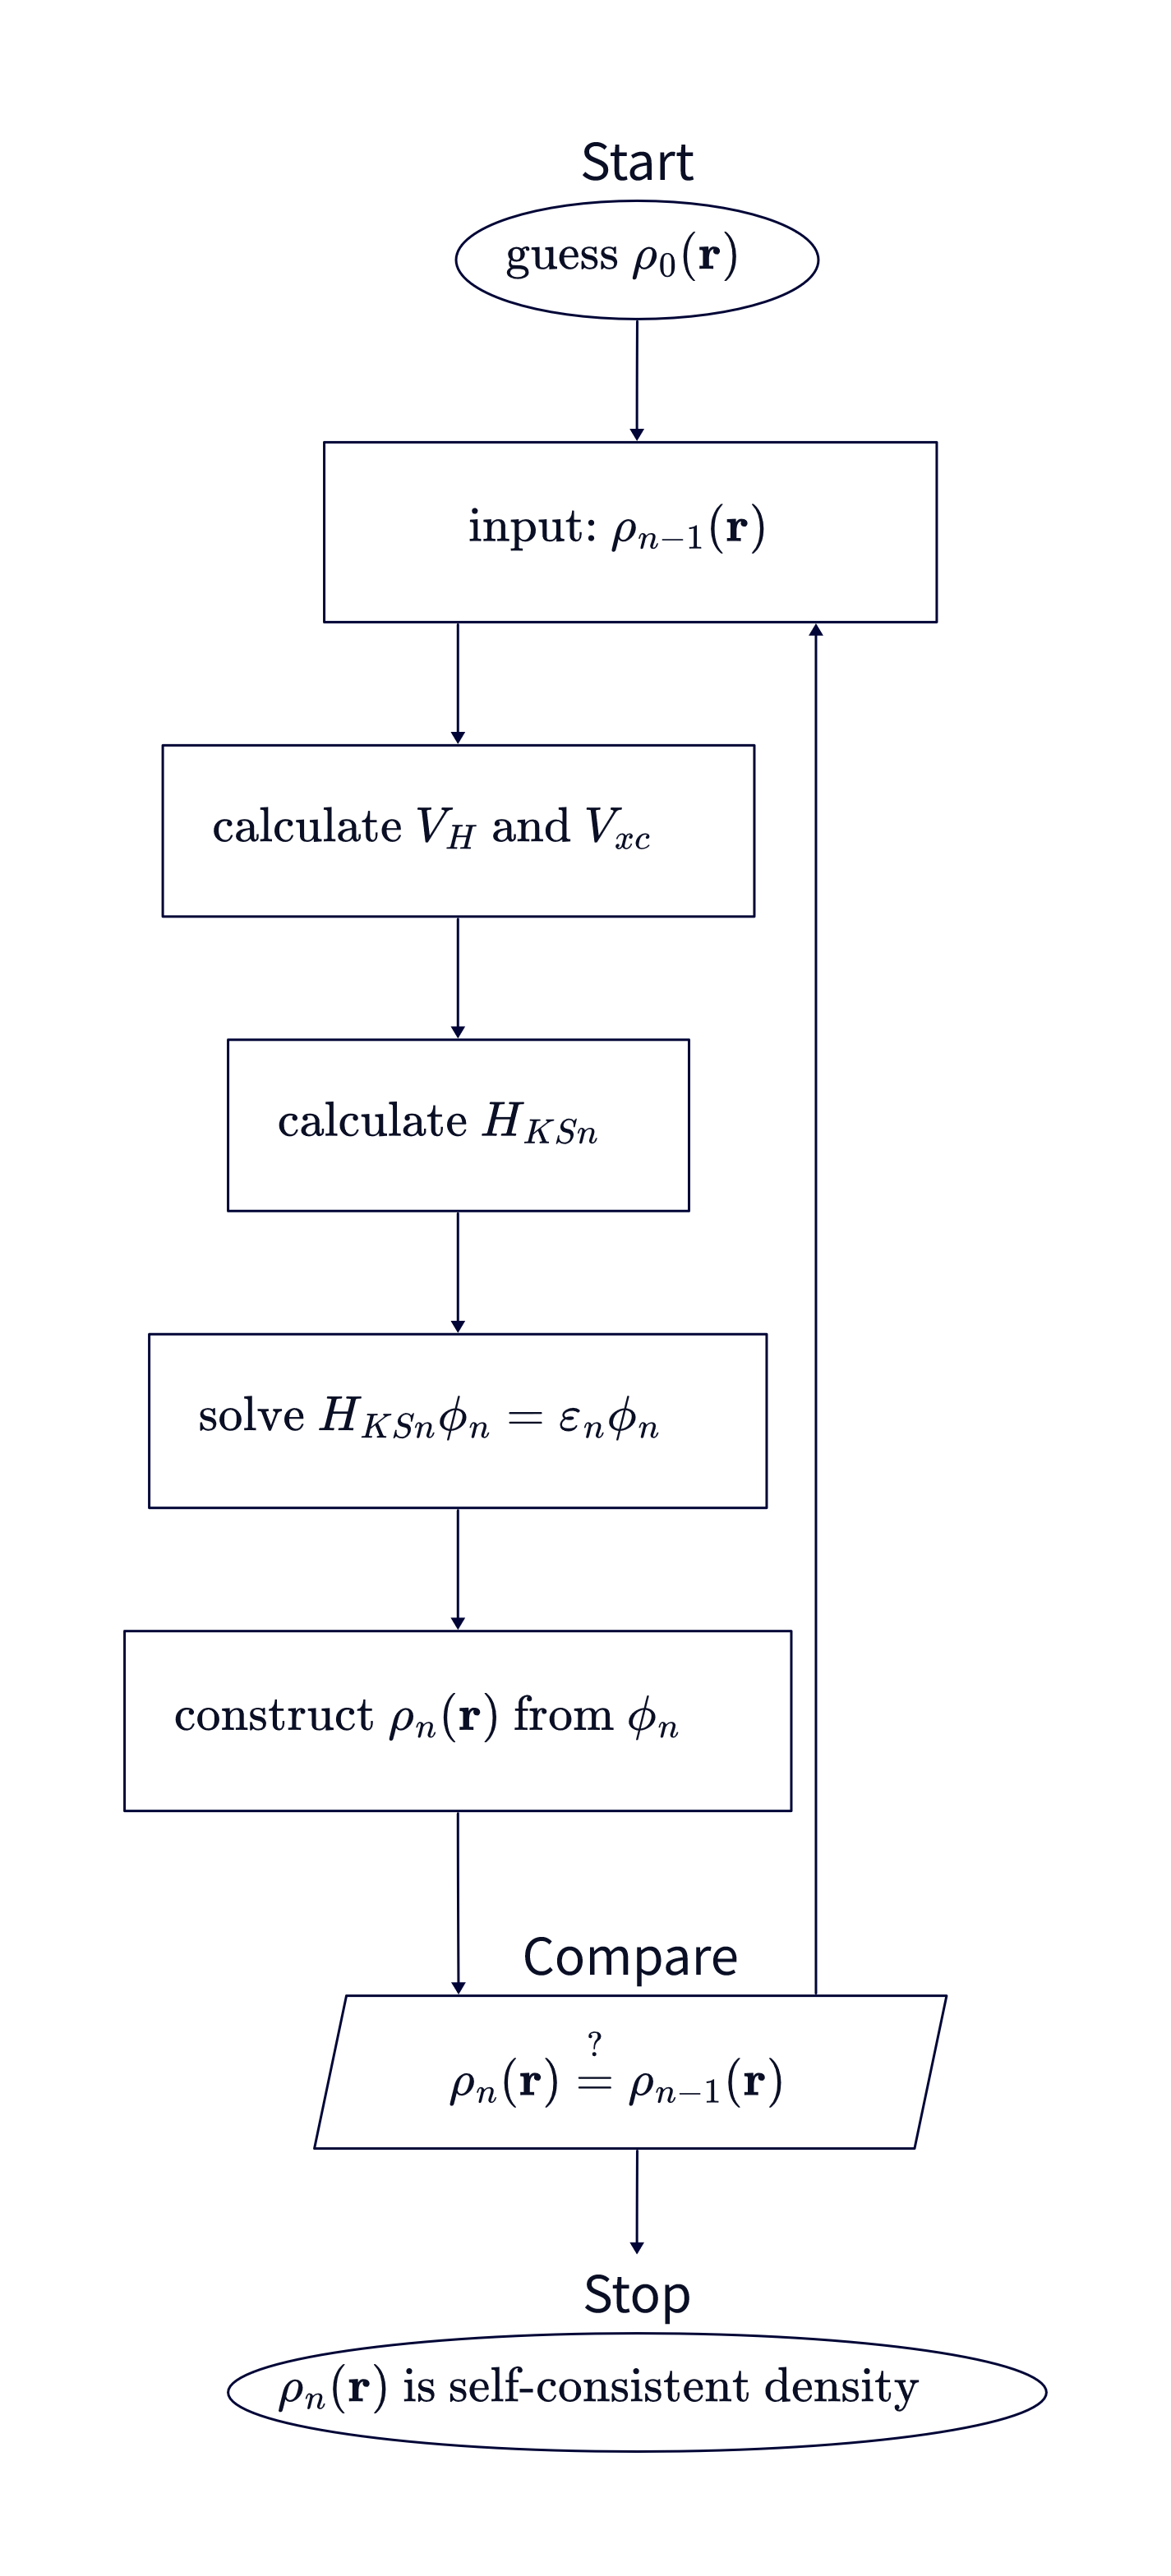
\includegraphics[width=7.3cm]{asset/self_consistency}
  \end{center}
  \caption{Flowchart for solving the self-consistent DFT problem.}
  \label{fig:self-consistency}
\end{figure}

\section{Machine Learning}

Until recently, classical molecular dynamics simulations based on empirical
force fields and \textit{ab initio} calculations were the only available
methods in computational physicists' toolbox. However, the rapid advent of
machine learning and artificial intelligence algorithms drastically changed
the landscape of physical simulations. When trained on large datasets of
atomic configurations and corresponding potential energies and forces,
ML models can reproduce the original data accurately, while still retaining
the linearly scaling computational cost of classical MD simulations. Although
ML methods are often quite data-demanding, their accuracy, scalability, and
transferability make them a very attractive alternative for various MD
applications.

\section{Deep Potential Molecular Dynamics}

The Deep Potential Molecular Dynamics (DeepMD) \parencite{Zhang_2018} method
uses neural networks for modeling many-body potentials and interatomic forces
to drive classical molecular dynamics. The neural network architectures used
by the DeepMD method are designed so that they preserve all the natural
symmetries in the problem. These models are trained on \textit{ab initio} data
and are capable of producing results that are essentially indistinguishable
from the original data while scaling linearly with the system size.

One of the most notable challenges in developing an efficient NN schema for
molecular dynamics is devising an input format that would preserve the
translational, rotational, and permutational symmetry of the system. The raw
atomic coordinates from MD simulations cannot be used directly, as they do not
exhibit these symmetries. Different ML models were proposed to address this
problem. For example, the Behler--Parrinello neural network (BPNN)
\parencite{PhysRevLett.98.146401} maps the coordinates onto a large set of
two- and three-body symmetry functions. Another proposed model,
gradient-domain machine learning (GDML)
\parencite{doi:10.1126/sciadv.1603015}, maps the coordinates onto the
eigenvalues of the Coulomb matrix. Both of these protocols are successful, but
they are also needlessly complicated, with their use-cases being rather
limited, as they do not come from a first-principles analysis of the modeling
problem, and it is not straightforward to extend them beyond simple systems.
The DeepMD methodology attempts to provide a more first principle-based
approach to overcome the limitations associated with auxiliary quantities like
the symmetry functions or the Coulomb matrix.

Consider a system of $N$ atoms, where the coordinates of these atoms can be
represented as a set of position vectors
$\{\mathbf{R}_1, \dots, \mathbf{R}_N\}$, with each
$\mathbf{R}_i \in \mathbb{R}^3$. DeepMD decomposes the total system energy $E$
into a sum of energy contributions from individual atoms,
\begin{equation}
  E = \sum_i^N E_i,
\end{equation}
where $i$ is an index of an individual atom. Atomic energy $E_i$ is fully
determined by the position of the $i$th atom and by the positions of its near
neighbours,
\begin{equation}
  E_i = E_{s(i)}(\mathbf{R}_i, \{\mathbf{R}_j \mid j \in  N_{R_C}(i)\}),
\end{equation}
where $N_{R_C}(i)$ denotes the index set of the neighbour atoms of atom $i$
within the cut-off radius $R_C$. $s(i)$ is the chemical species of atom $i$.
For reasons discussed above, it is less than optimal to use the position
vector data $\mathbf{R}_i, \{\mathbf{R}_j \mid j \in  N_{R_C}(i)\}$ when
modeling the function $E_{s(i)}$ with DNN. Thus, the DeepMD method introduces
a mapping from position vectors to "descriptors" of atomic chemical
environment, that better capture the underlying symmetries.

To construct the descriptor for atom $i$, we first calculate the relative
positions of its neighbouring atoms,
\begin{equation}
  \mathbf{R}_{ij} = \mathbf{R}_j - \mathbf{R}_i.
\end{equation}
The coordinate of the relative position $R_{ij}$ under the lab reference frame
$\{\mathbf{e}_x^0, \mathbf{e}_y^0, \mathbf{e}_z^0\}$ is denoted by
$(x_{ij}^0, y_{ij}^0, z_{ij}^0)$, such that
\begin{equation}
  \mathbf{R}_{ij} = x_{ij}^0 \mathbf{e}_x^0 + y_{ij}^0 \mathbf{e}_y^0
    + z_{ij}^0 \mathbf{e}_z^0.
\end{equation}
Both representations $\mathbf{R}_{ij}$ and $(x_{ij}^0, y_{ij}^0, z_{ij}^0)$
preserve the translational symmetry. The rotational symmetry is captured by
constructing a local frame of reference and using it to express the
coordinates of neighbouring atoms. We first pick atoms with indices $a(i)$ and
$b(i)$ from the neighbours $N_{R_C}(i)$ by certain user-specified rules. The
local reference frame $\{\mathbf{e}_{i1}, \mathbf{e}_{i2}, \mathbf{e}_{i3} \}$
of atom $i$ is then constructed by
\begin{align}
  \mathbf{e}_{i1} = \mathbf{e}(\mathbf{R}_{ia(i)}), \\
  \mathbf{e}_{i2} = \mathbf{e}\left(
    \mathbf{R}_{ib(i)} -
    (\mathbf{R}_{i b(i)} \cdot \mathbf{e}_{i1}) \mathbf{e}_{i1}
  \right), \\
  \mathbf{e}_{i3} = \mathbf{e}_{i1} \times \mathbf{e}_{i2},
\end{align}
where $\mathbf{e}(\mathbf{R})$ denotes the normalized vector of $\mathbf{R}$,
such that $\mathbf{e}(\mathbf{R}) = \mathbf{R} / |\mathbf{R}|$. The local
coordinate $(x_{ij}, y_{ij}, z_{ij})$ is then calculated from the lab
coordinate $(x_{ij}^0, y_{ij}^0, z_{ij}^0)$ through the transformation
\begin{equation}
  (x_{ij}, y_{ij}, z_{ij}) = (x_{ij}^0, y_{ij}^0, z_{ij}^0) \cdot
    \mathcal{R}(\mathbf{R}_{i a(i)}, \mathbf{R}_{i b(i)}),
\end{equation}
where
\begin{equation}
  \mathcal{R}(\mathbf{R}_{i a(i)}, \mathbf{R}_{i b(i)}) =
    [\mathbf{e}_{i1}, \mathbf{e}_{i2}, \mathbf{e}_{i3}]
\end{equation}
is the rotation matrix with the columns being the local reference frame
vectors. The descriptive information of atom $i$ given by neighboring atom $j$
is then obtained by using either both the radial and angular information or
only the radial information
\begin{equation}
  \{D_{ij}\} = \begin{cases}
    \left\{
      \frac{1}{R_{ij}},
      \frac{x_{ij}}{R_{ij}},
      \frac{y_{ij}}{R_{ij}},
      \frac{z_{ij}}{R_{ij}}
    \right\}, & \text{full information;} \\
    \left\{\frac{1}{R_{ij}}\right\}, & \text{radial-only information.}
  \end{cases}
  \label{eq:descriptor}
\end{equation}
The order of the neighbour indices $j$ in $\{D_{ij}\}$ is fixed by sorting
them first by their chemical species and then, within each chemical species,
according to their inverse distances to the atom $i$, i.e., $1/R_{ij}$. The
permutational symmetry is naturally preserved in this way. This is the full
procedure for constructing the mapping from atomic positions to descriptors,
which is denoted by
\begin{equation}
  \mathbf{D}_i = \mathbf{D}_i(
    \mathbf{R}_i, \{\mathbf{R}_j \mid j \in  N_{R_C}(i)\}
  ).
\end{equation}
The descriptors $\mathbf{D}_i$ preserve the translational, rotational, and
permutational symmetries and are passed to a DNN to evaluate the atomic
energies. This process can be mathematically expressed as
\begin{equation}
  E_{s(i)} = \mathcal{N}_{s(i)}(\mathbf{D}_{i}),
  \label{eq:dnn}
\end{equation}
The DNN used by DeepMD method is a feed forward neural network with multiple
hidden layers, where each layer transforms the input data $\mathbf{d}_i^{p-1}$
from the previous layer into $\mathbf{d}_i^{p}$ and passes them as an input
to the next layer. The transformation consists of a linear and a non-linear
step, i.e.
\begin{equation}
  \mathbf{d}_{i}^{p} = \varphi \left(
    \mathbf{W}_{s(i)}^p \mathbf{d}_i^{p-1} + \mathbf{b}^p_{s(i)}
  \right),
\end{equation}
where $\varphi$ represents the non-linear function and $\mathbf{W}_{s(i)}^p$
and $\mathbf{b}^p_{s(i)}$ are free parameters of the linear transformation to
be optimize by the training process. In order to determine the unknown
parameters ${\mathbf{W}{s}^p, \mathbf{b}s^p}$ of the linear transformation, a
loss function $L$ is minimized during the training process. This loss
function is calculated by taking a weighted sum of mean square errors of the
predictions made by the DNN. Specifically, the loss function
$L(p_\epsilon, p_f, p_\xi)$ is defined as follows:
\begin{equation}
  L(p_\epsilon, p_f, p_\xi) = \frac{p_\epsilon}{N} \Delta E^2 +
  \frac{p_f}{3N} \sum_i |\Delta \mathbf{F}_i|^2
  + \frac{p_\xi}{9N} ||\Delta \Xi||^2,
\end{equation}
where $\Delta E$, $\Delta \mathbf{F}_i$ and $\Delta \Xi$ denote root mean
square (RMS) error in energy, force, and virial, respectively. The weights
$p_\epsilon$, $p_f$ and $p_\xi$ are varying during the learning process. Their
dependence on the learning step $t$ is defined as
\begin{equation}
  p(t) = p^\text{limit} \left[1 - \frac{r_l(t)}{r_l^0}\right]
  + p^\text{start} \left[\frac{r_l(t)}{r_l^0}\right],
  \label{eq:loss-weight}
\end{equation}
where $r_l(t)$ and $r_l^0$ are the learning rate at training step $t$ and the
learning rate ate the beginning, respectively. The prefactors $p^\text{limit}$
and $p^\text{start}$ are specified by the user configuration. It is easy to
observe that as the learning process starts the factor $\frac{r_l(t)}{r_l^0}$
tends to $1$ and thus the value of $p(t)$ tends to $p^\text{start}$. When the
learning process ends, the factor $1 - \frac{r_l(t)}{r_l^0}$ tends to $1$ and
thus the value of $p(t)$ tends to $p^\text{limit}$. By tuning these
parameters a user can precisely specify what physical properties of the system
should the model be learning to predict at different stages of the learning
process. The learning rate $r_l(t)$ function is in our case given by
\begin{equation}
  r_l(t) = r_l^0 \cdot d_r^{t/d_s},
  \label{eq:learning-rate}
\end{equation}
where $d_r$ and $d_s$ are the decay rate and decay steps, respectively. The
decay rate $d_r$ is required to be less than 1.
